\subsection{Схемы телескопов}
Телескопв по своей оптической схеме делятся на 3 типа:
\begin{enumerate}
\item Рефлекторы или диоптрические
\item Рефракторы или катаптрические
\item Катадиоптрические
\end{enumerate}

\term{Рефлектор} (зеркальный телескоп)~---  оптический телескоп, использующий в качестве светособирающего элемента зеркало.

\term{Рефрактор} (линзовый телескоп)~---  оптический телескоп, в котором для собирания света используется система линз.

\term{Катадиоптрический} (зеркально-линзовый) \textit{телескоп}~--- оптический телескоп, в котором используется как система линз, так и зеркал.

\begin{figure}
	\centering
	\begin{subfigure}{0.49\textwidth}
		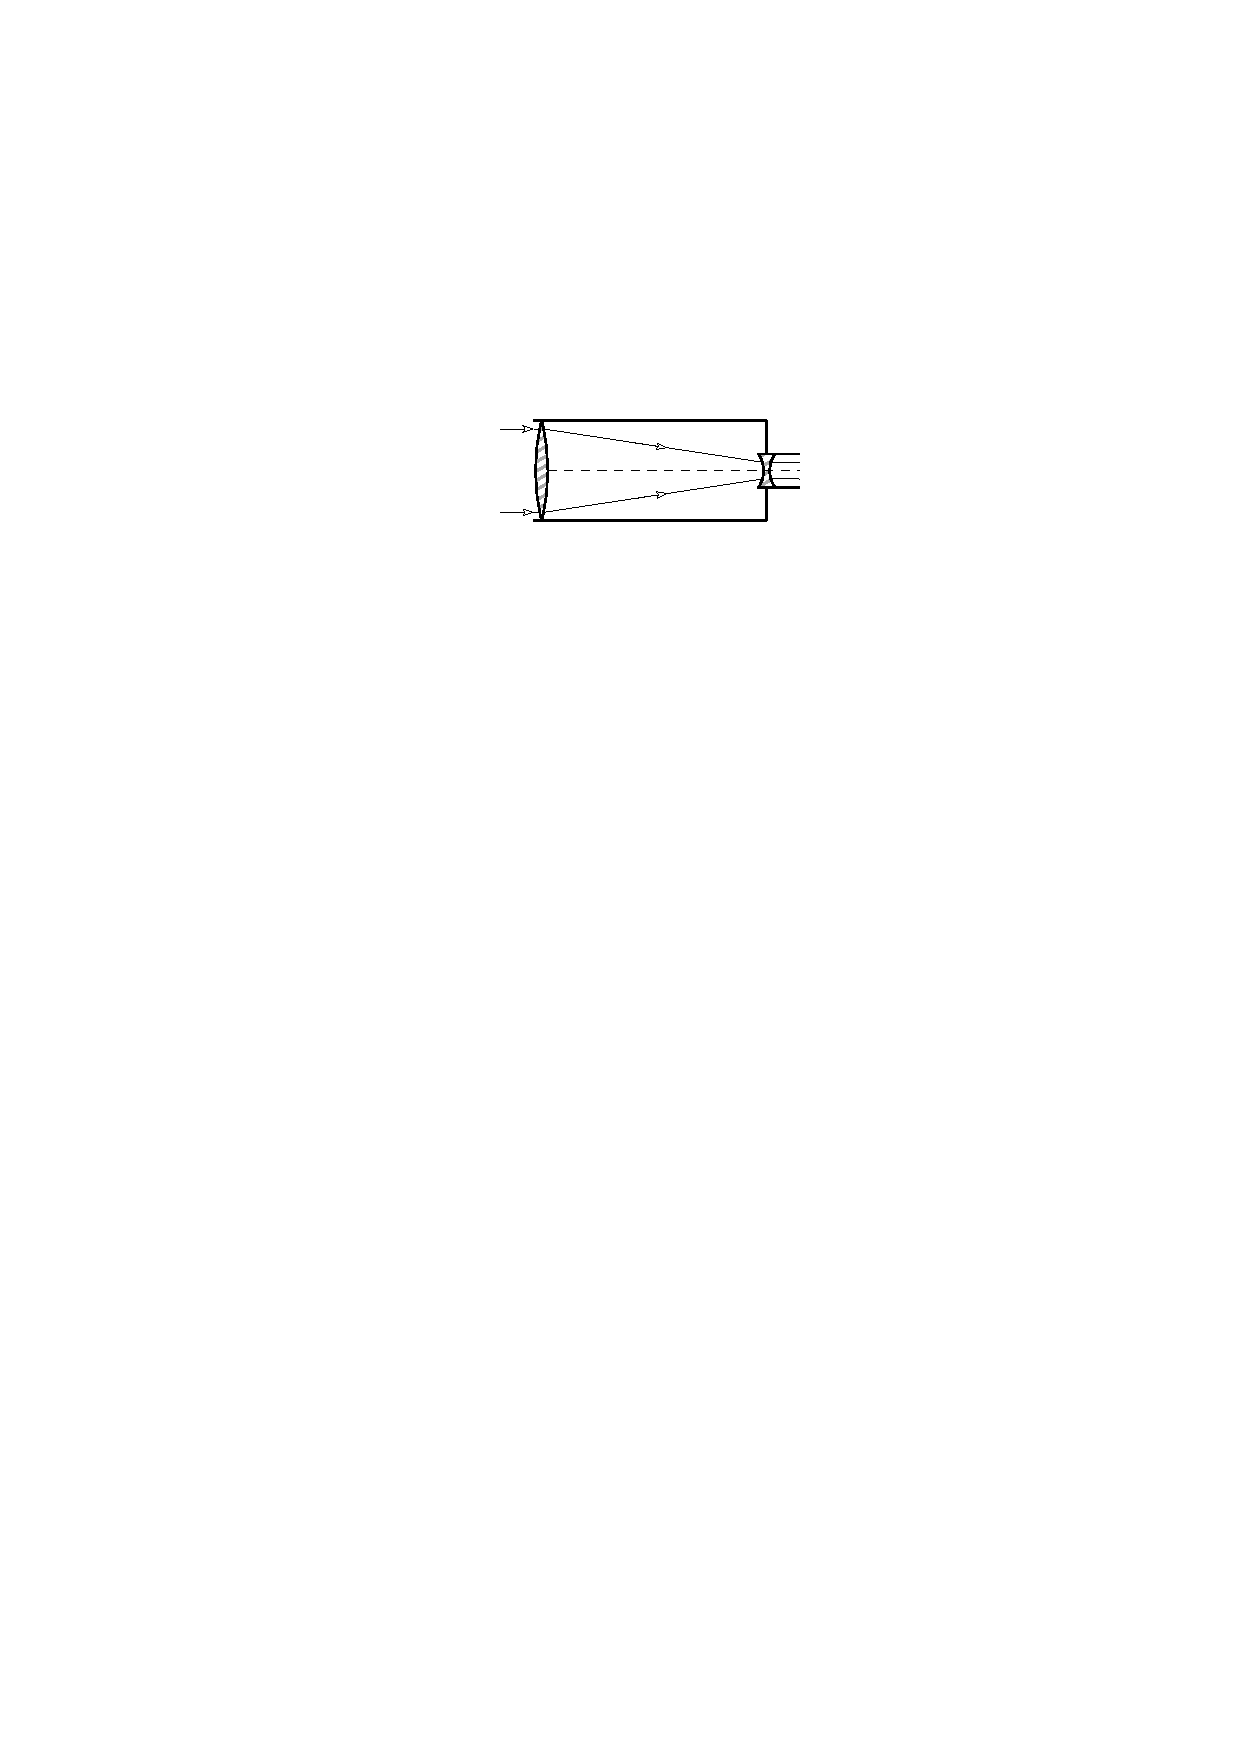
\includegraphics[width = \textwidth]{Galiley}
		\caption{\textit{Рефрактор системы Галилея}}
	 \end{subfigure}
	 \hfill
	\begin{subfigure}{0.49\textwidth}
		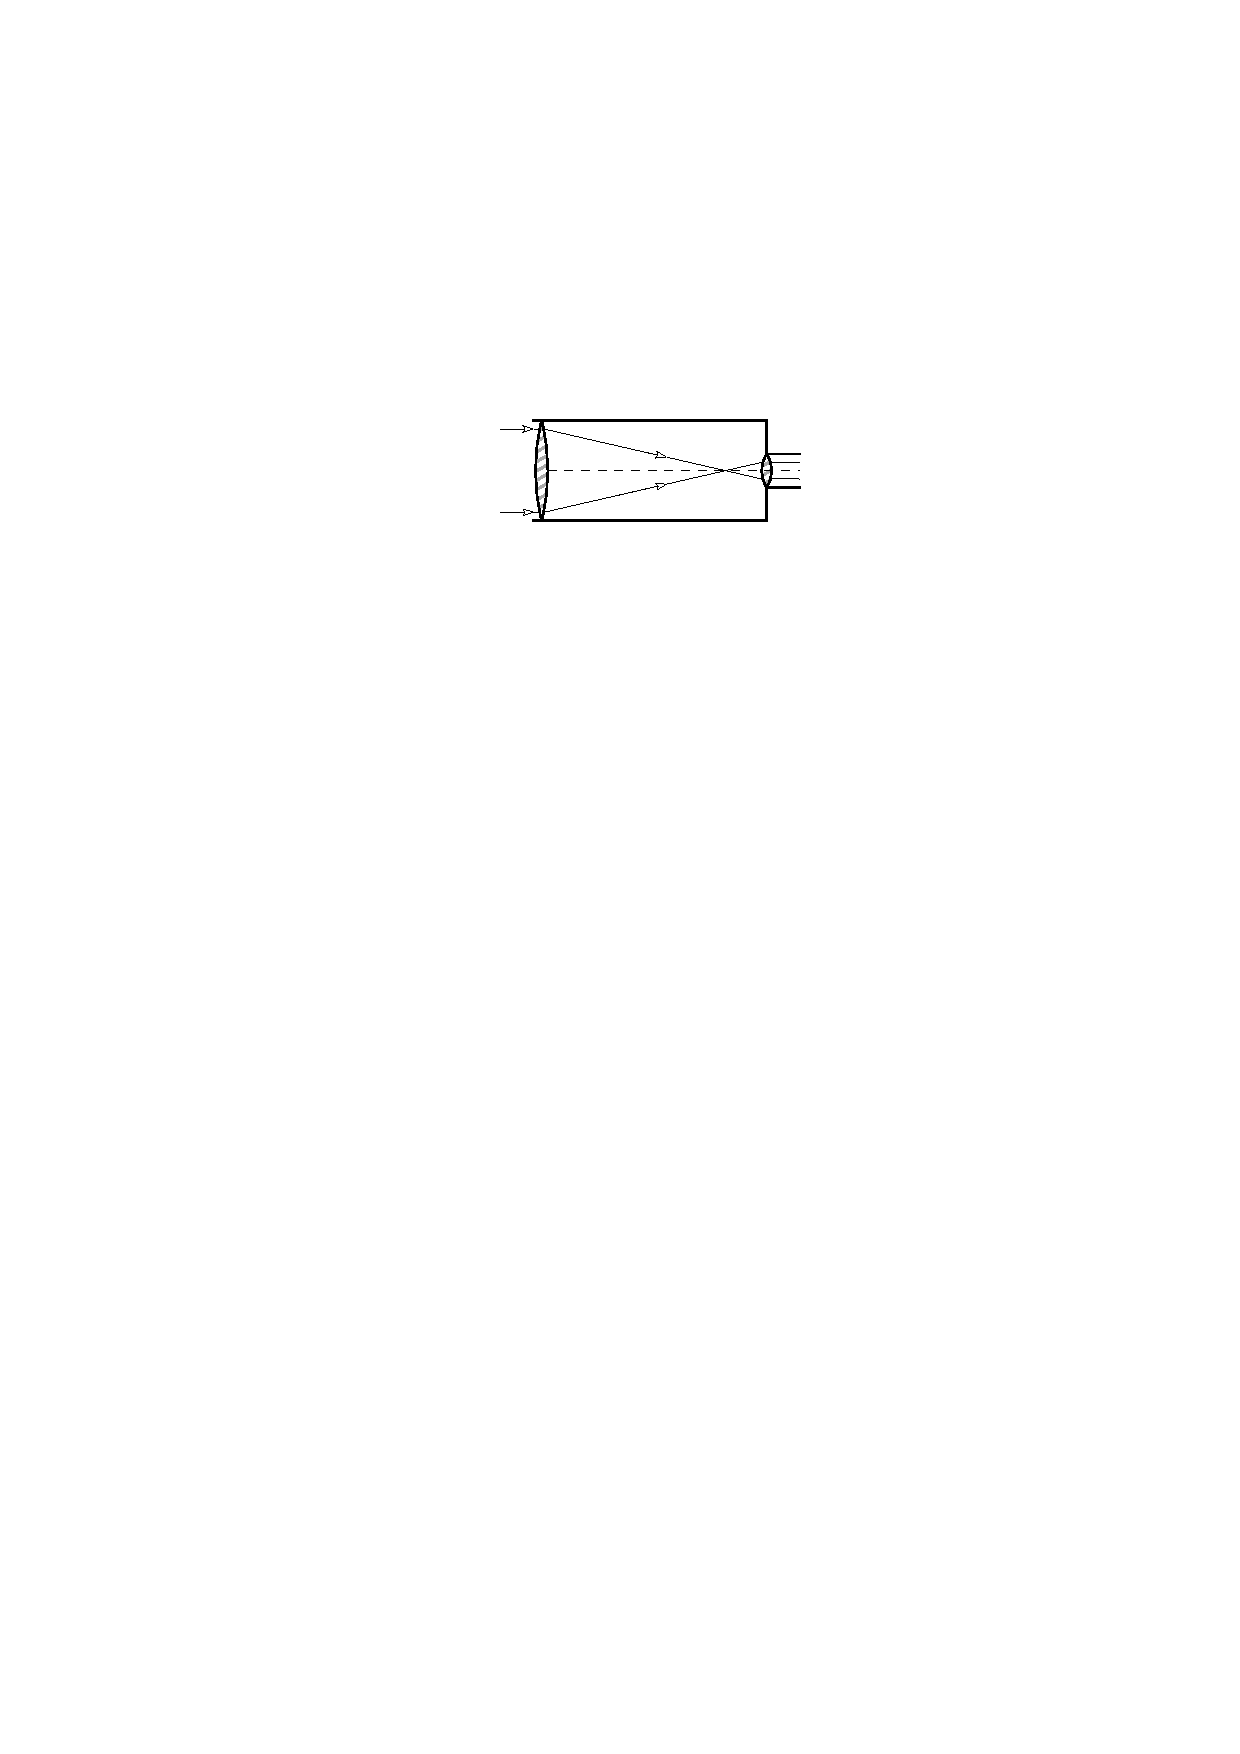
\includegraphics[width = \textwidth]{Kepler}
		\caption{\textit{Рефрактор системы Кеплера} \label{Kepler}}
	 \end{subfigure}
	 
	\begin{subfigure}{0.49\textwidth}
		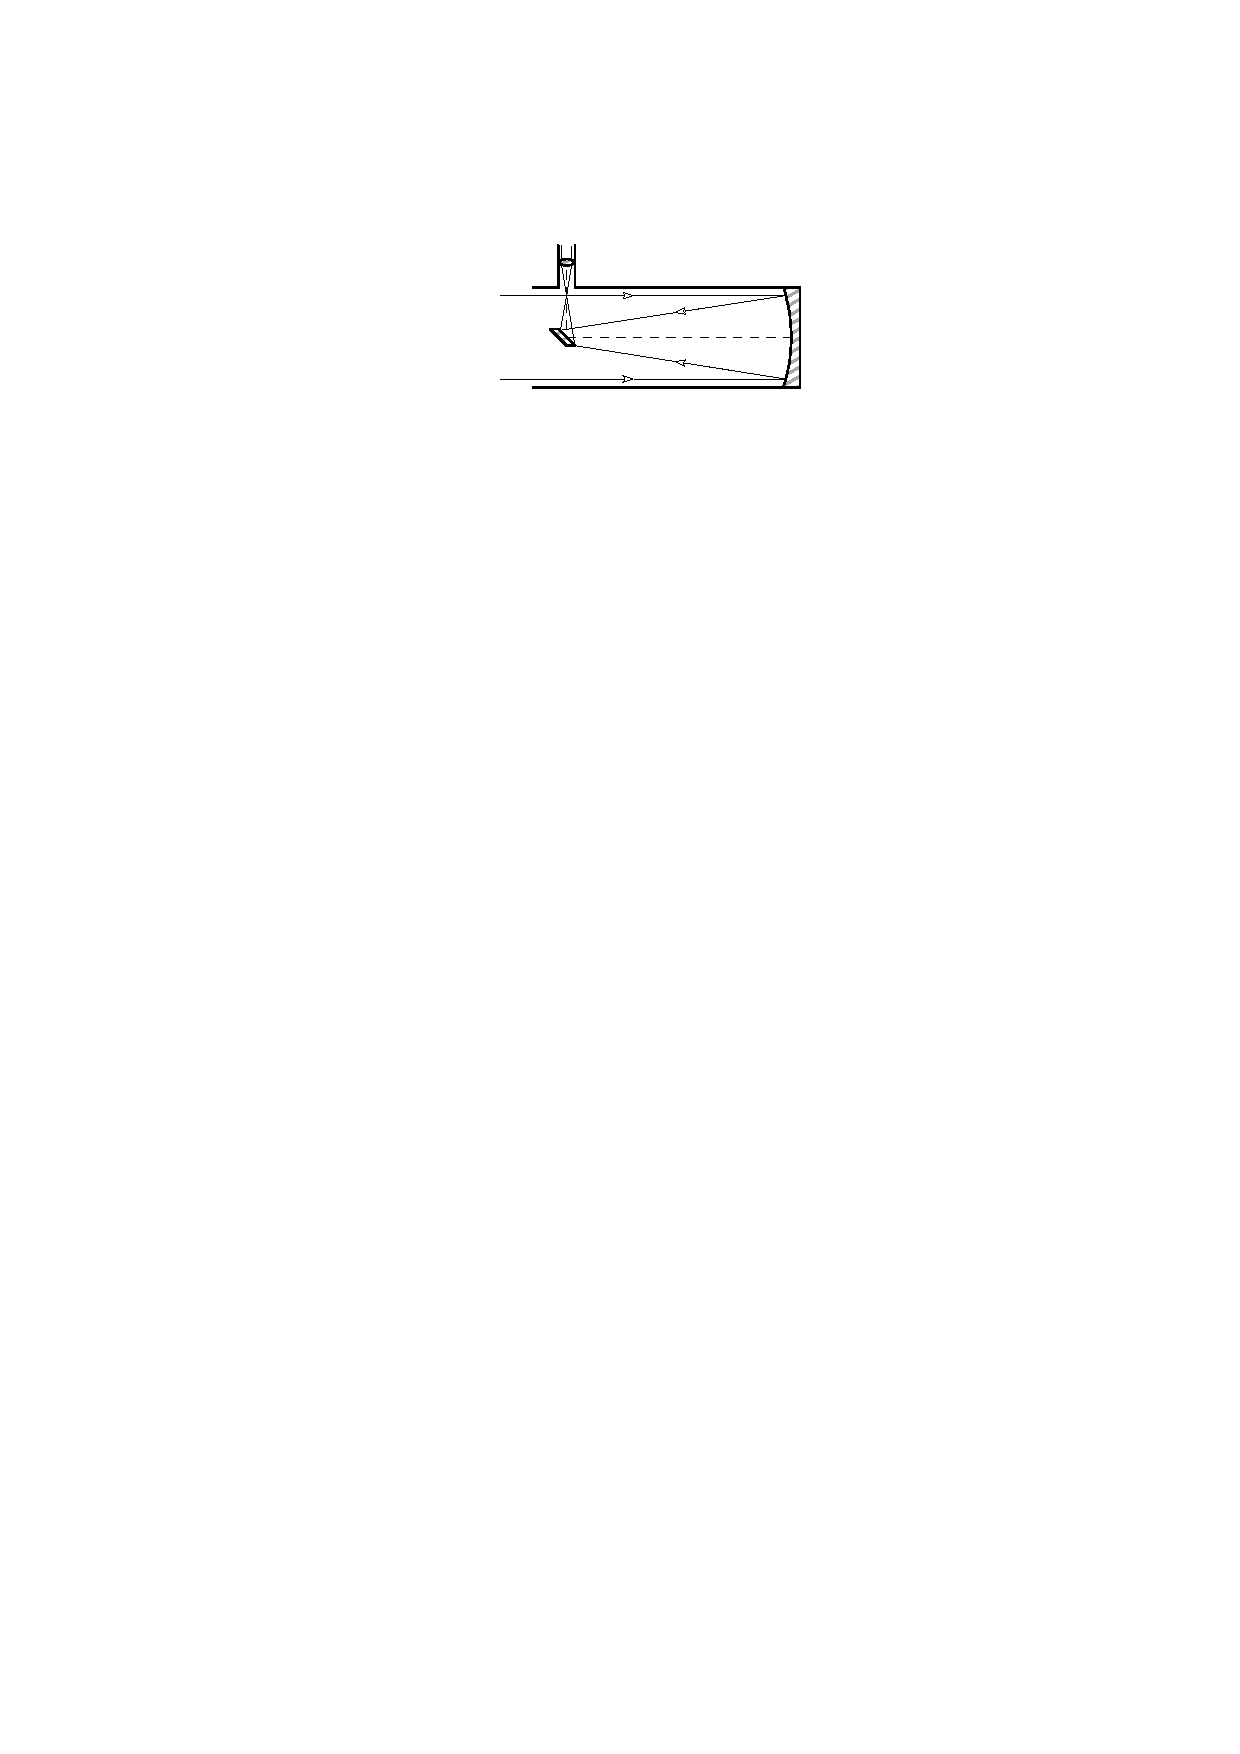
\includegraphics[width = \textwidth]
	{Newton.pdf}
	\caption{\textit{Рефлектор системы Ньютона} \label{Newton}}
	 \end{subfigure}
	 \hfill
	 \begin{subfigure}{0.49\textwidth}
		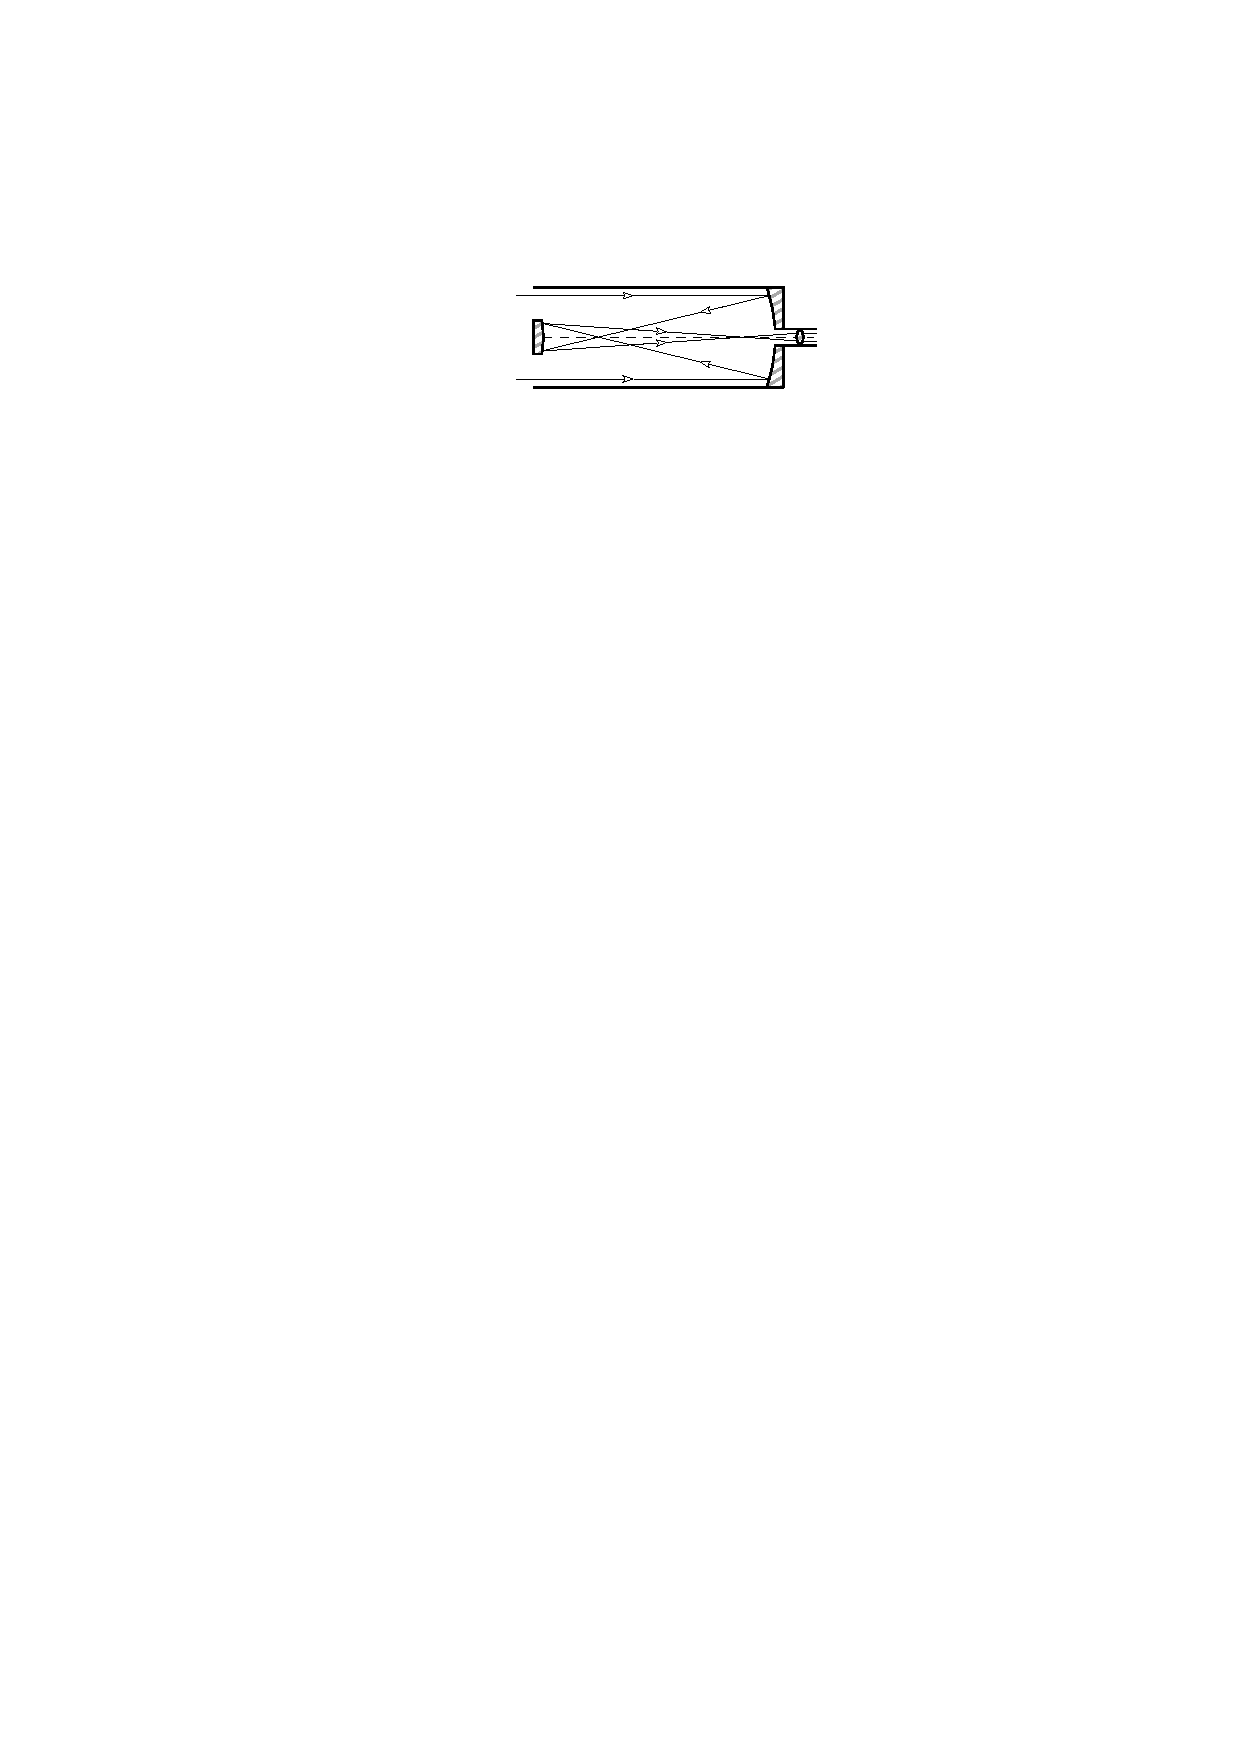
\includegraphics[width = \textwidth]
	{Gregory.pdf}
	\caption{\textit{Рефлектор системы Грегори} \label{Gregory}}
	 \end{subfigure}
	 
	 \begin{subfigure}{0.49\textwidth}
		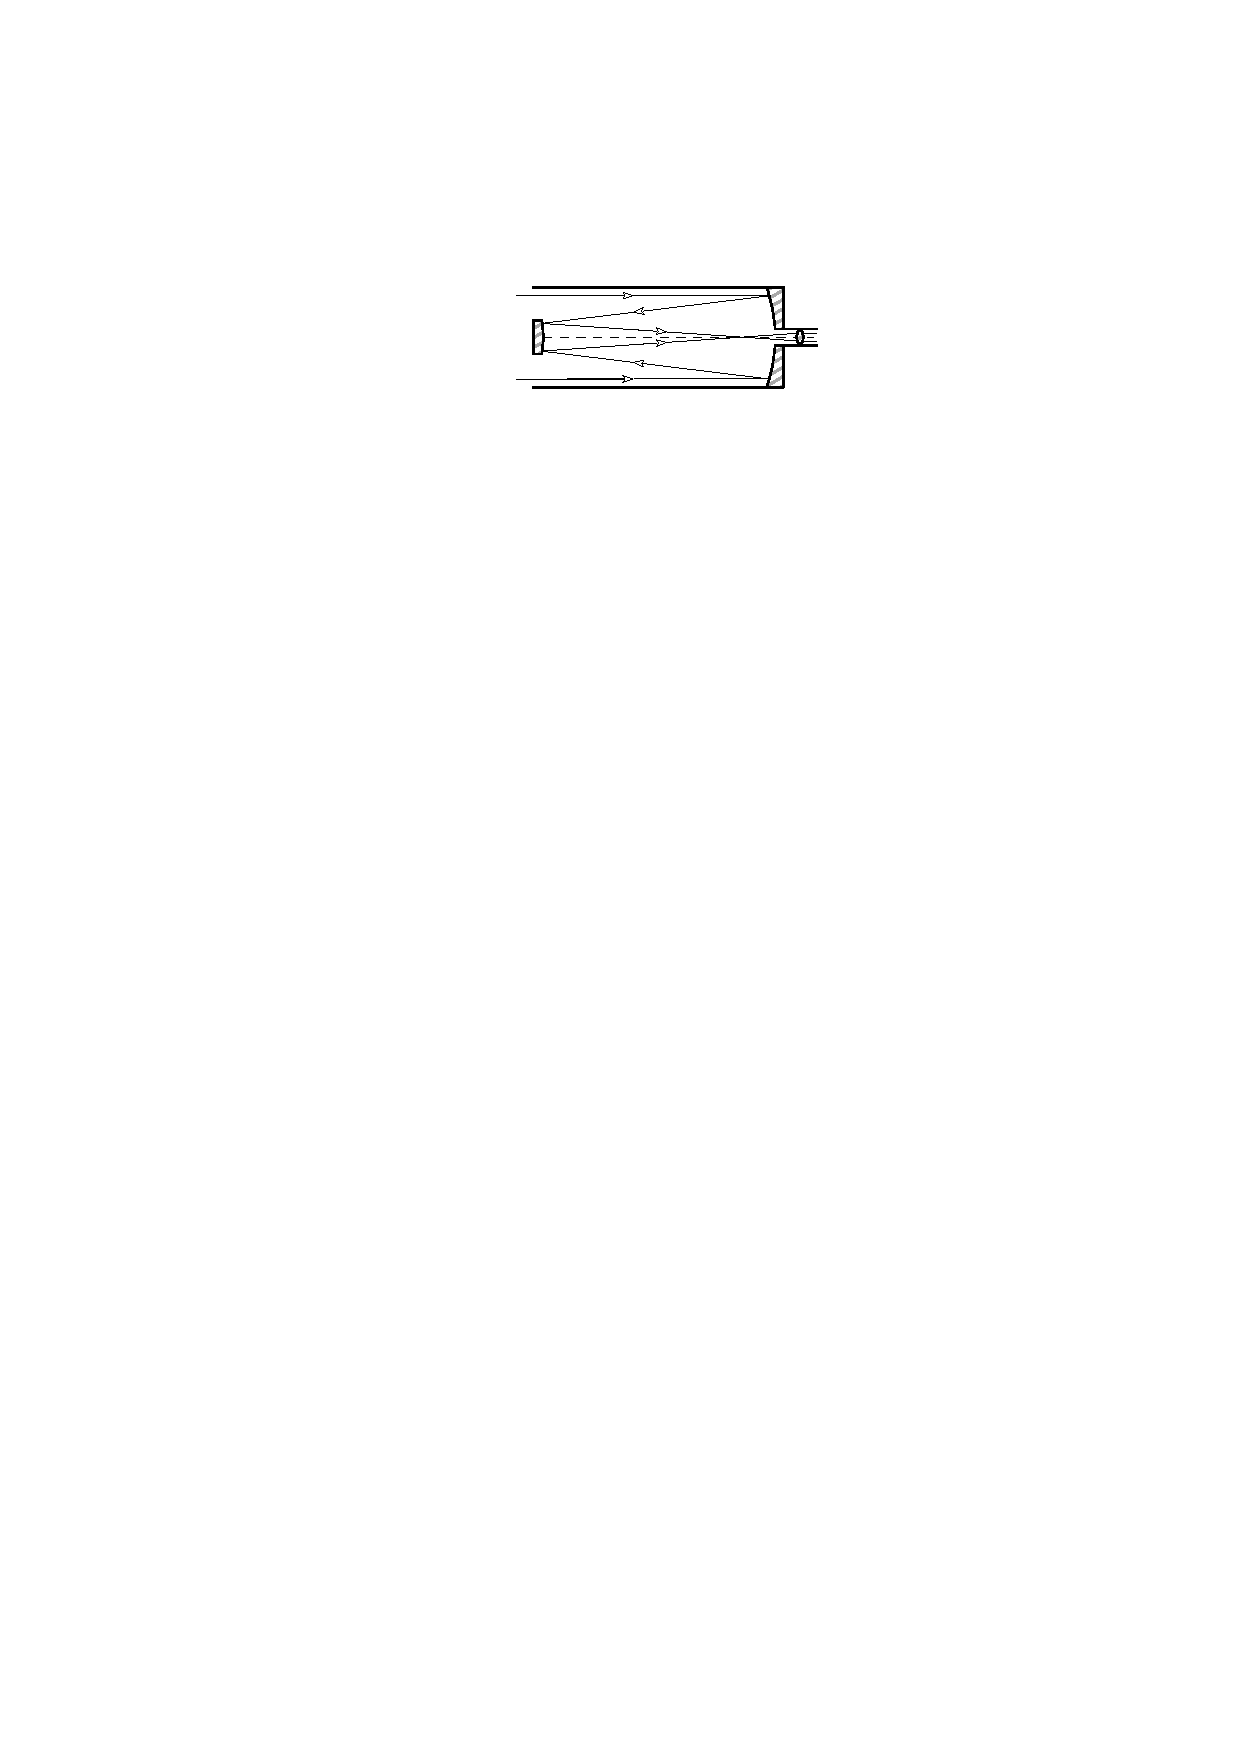
\includegraphics[width = \textwidth]
	{Cassigren.pdf}
	\caption{\textit{Рефлектор системы Кассигрена}}
	 \end{subfigure}
	 \hfill
	 \begin{subfigure}{0.49\textwidth}
		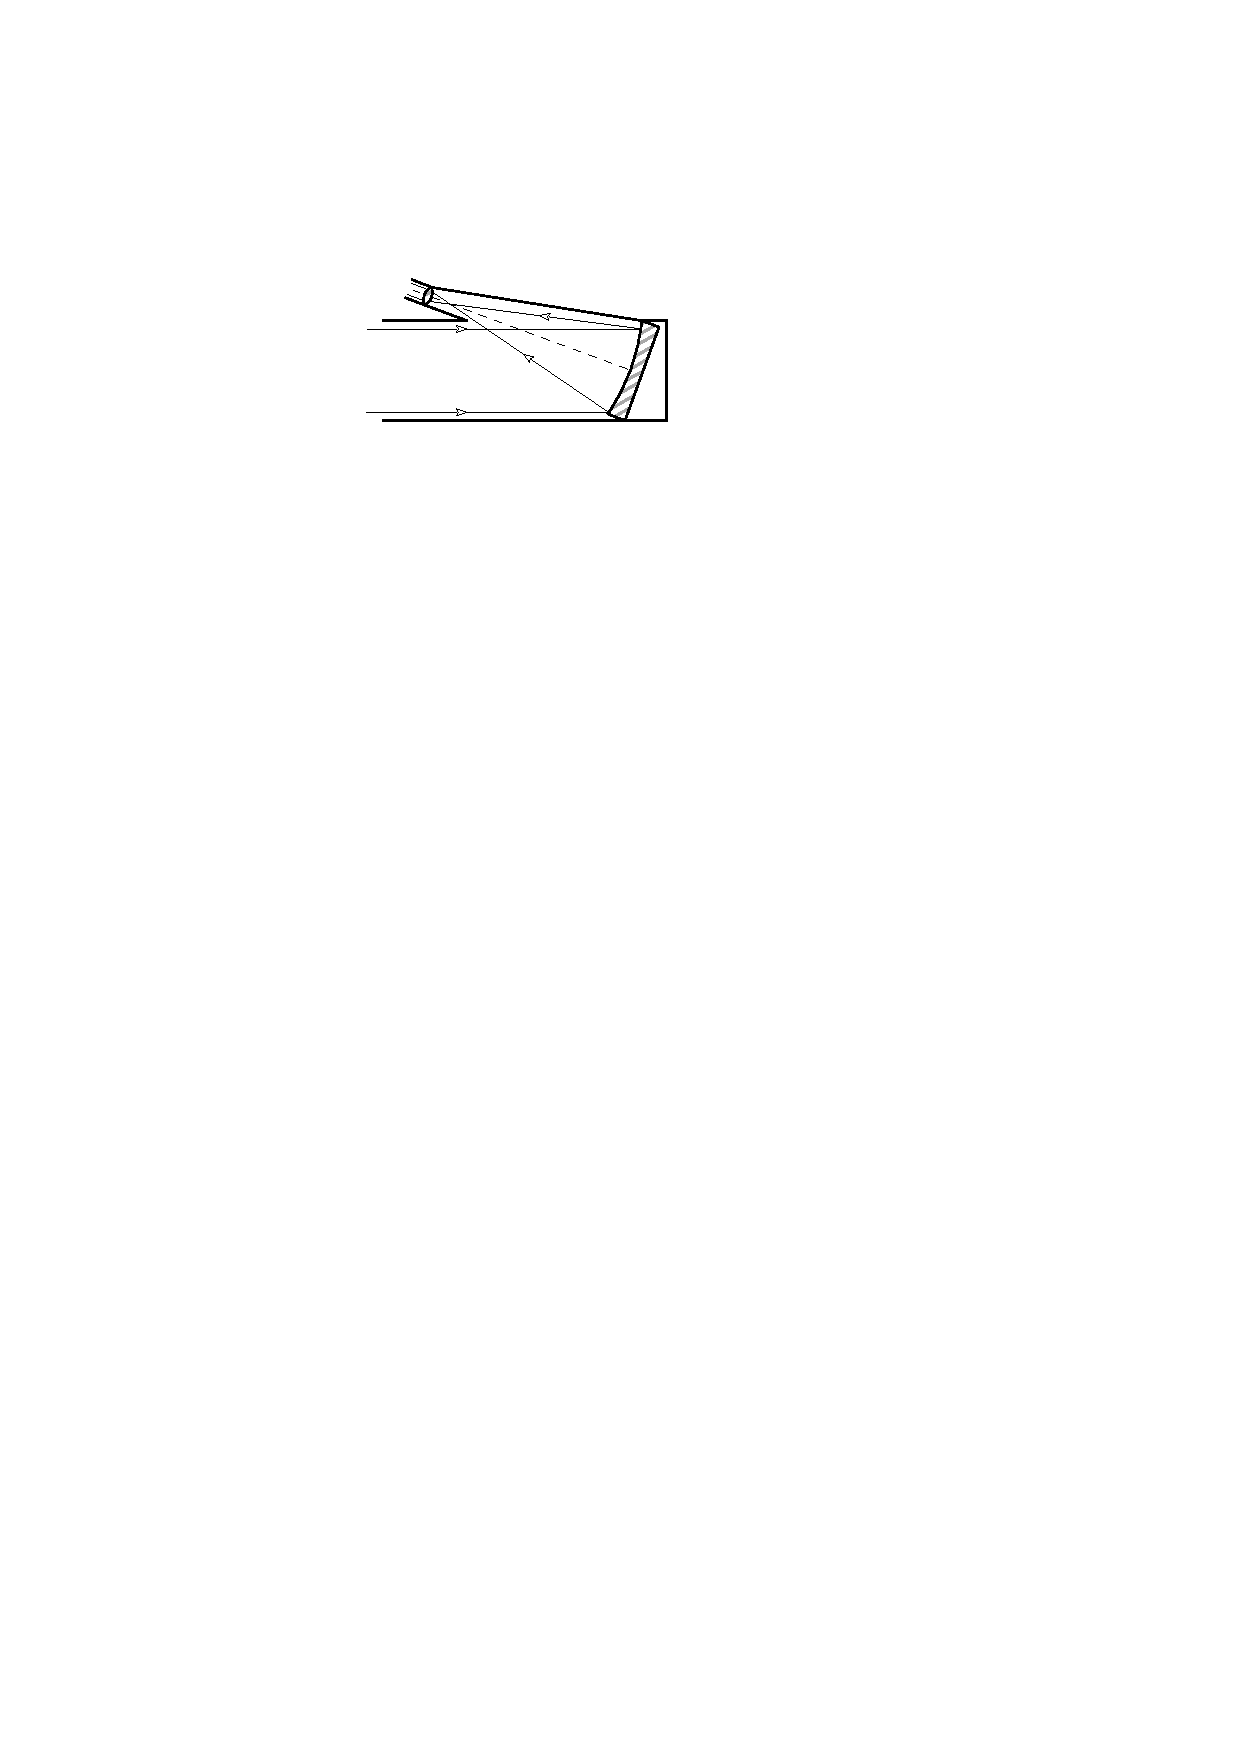
\includegraphics[width = \textwidth]
	{Lomonosov.pdf}
	\caption{\textit{Рефлектор системы Ломоносова}}
	 \end{subfigure}
\end{figure}

